\documentclass[12pt]{article}

\usepackage{amsmath, mathtools}
\usepackage{amsfonts}
\usepackage{amssymb}
\usepackage{graphicx}
\usepackage{colortbl}
\usepackage{xr}
\usepackage{hyperref}
\usepackage{longtable}
\usepackage{xfrac}
\usepackage{tabularx}
\usepackage{float}
\usepackage{siunitx}
\usepackage{booktabs}
\usepackage{caption}
\usepackage{pdflscape}
\usepackage{afterpage}

\usepackage[round]{natbib}

%\usepackage{refcheck}

\hypersetup{
    bookmarks=true,         % show bookmarks bar?
      colorlinks=true,       % false: boxed links; true: colored links
    linkcolor=red,          % color of internal links (change box color with 
linkbordercolor)
    citecolor=green,        % color of links to bibliography
    filecolor=magenta,      % color of file links
    urlcolor=cyan           % color of external links
}

%% Comments

\usepackage{color}

\newif\ifcomments\commentstrue

\ifcomments
\newcommand{\authornote}[3]{\textcolor{#1}{[#3 ---#2]}}
\newcommand{\todo}[1]{\textcolor{red}{[TODO: #1]}}
\else
\newcommand{\authornote}[3]{}
\newcommand{\todo}[1]{}
\fi

\newcommand{\wss}[1]{\authornote{blue}{SS}{#1}} 
\newcommand{\plt}[1]{\authornote{magenta}{TPLT}{#1}} %For explanation of the template
\newcommand{\an}[1]{\authornote{cyan}{Author}{#1}}

%% Common Parts

\newcommand{\progname}{Diagnose} % PUT YOUR PROGRAM NAME HERE %Every program
                                % should have a name


% For easy change of table widths
\newcommand{\colZwidth}{1.0\textwidth}
\newcommand{\colAwidth}{0.13\textwidth}
\newcommand{\colBwidth}{0.82\textwidth}
\newcommand{\colCwidth}{0.1\textwidth}
\newcommand{\colDwidth}{0.05\textwidth}
\newcommand{\colEwidth}{0.8\textwidth}
\newcommand{\colFwidth}{0.17\textwidth}
\newcommand{\colGwidth}{0.5\textwidth}
\newcommand{\colHwidth}{0.28\textwidth}

% Used so that cross-references have a meaningful prefix 
\newcounter{defnum} %Definition Number
\newcommand{\dthedefnum}{GD\thedefnum}
\newcommand{\dref}[1]{GD\ref{#1}}
\newcounter{datadefnum} %Datadefinition Number
\newcommand{\ddthedatadefnum}{DD\thedatadefnum}
\newcommand{\ddref}[1]{DD\ref{#1}}
\newcounter{theorynum} %Theory Number
\newcommand{\tthetheorynum}{T\thetheorynum}
\newcommand{\tref}[1]{T\ref{#1}}
\newcounter{tablenum} %Table Number
\newcommand{\tbthetablenum}{T\thetablenum}
\newcommand{\tbref}[1]{TB\ref{#1}}
\newcounter{assumpnum} %Assumption Number
\newcommand{\atheassumpnum}{P\theassumpnum}
\newcommand{\aref}[1]{A\ref{#1}}
\newcounter{goalnum} %Goal Number
\newcommand{\gthegoalnum}{P\thegoalnum}
\newcommand{\gsref}[1]{GS\ref{#1}}
\newcounter{instnum} %Instance Number
\newcommand{\itheinstnum}{IM\theinstnum}
\newcommand{\iref}[1]{IM\ref{#1}}
\newcounter{reqnum} %Requirement Number
\newcommand{\rthereqnum}{P\thereqnum}
\newcommand{\rref}[1]{R\ref{#1}}
\newcounter{nreqnum} %NRequirement Number
\newcommand{\nrthereqnum}{NP\thenreqnum}
\newcommand{\nrref}[1]{NR\nref{#1}}
\newcounter{lcnum} %Likely change number
\newcommand{\lthelcnum}{LC\thelcnum}
\newcommand{\lcref}[1]{LC\ref{#1}}
\newcounter{ucnum} %Likely change number
\newcommand{\ltheucnum}{UC\thelcnum}
\newcommand{\ucref}[1]{UC\ref{#1}}

\usepackage{fullpage}

\begin{document}

\title{Software Requirements Specification for diagnosis-AIDs\progname: Medical 
Diagnosis Prediction Tool for Acquired immunodeficiency syndrome (AIDS)} 
\author{Andrea Clemeno}
\date{\today}
	
\maketitle

~\newpage

\pagenumbering{roman}

\tableofcontents

~\newpage

\section*{Revision History}

\begin{tabularx}{\textwidth}{p{3cm}p{2cm}X}
\toprule {\bf Date} & {\bf Version} & {\bf Notes}\\
\midrule
October 10 2020 & 1.0 & Initial Draft of SRS\\
%Date 2 & 1.1 & Notes\\
\bottomrule
\end{tabularx}

~\newpage

\section{Reference Material}

This section records information for easy reference.

\subsection{Table of Units}

Throughout this document SI (Syst\`{e}me International d'Unit\'{e}s) is employed
as the unit system.  In addition to the basic units, several derived units are
used as described below.  For each unit, the symbol is given followed by a
description of the unit and the SI name.
~\newline

\renewcommand{\arraystretch}{1.2}
\begin{table}[ht]
\begin{center}
 \noindent \begin{tabular}{l l l}
    \toprule		
    \textbf{symbol} & \textbf{unit} & \textbf{SI}\\
    \midrule 
    \si{\metre} & length & metre\\
    \si{\kilogram} & mass	& kilogram\\
    \si{\second} & time & second\\
    \si{\celsius} & temperature & centigrade\\
    \bottomrule
  \end{tabular}
  \end{center}
  	\caption{Table of Units}
\end{table}

 

\subsection{Table of Symbols}

The table that follows summarizes the symbols used in this document along with
their units. The symbols are listed in alphabetical order.

\begin{table}[ht]
\renewcommand{\arraystretch}{1.2}
%\noindent \begin{tabularx}{1.0\textwidth}{l l X}
\noindent \begin{longtable*}{l l p{12cm}} \toprule
\textbf{symbol} & \textbf{unit} & \textbf{description}\\
\midrule 
$A_1$ & \si[per-mode=symbol] {$1 / 10^{-3}m^3}$} & initial amount of substance
\\
$A_2$ & \si[per-mode=symbol]{$1 / 10^{-3}m^3}$} & amount of substance at second 
instance 
\\ 
$isDecaying$ & - & requirement of decaying rate of change
\\
$N_0$ & \si[per-mode=symbol] {\mol} & initial amount of substance
\\
$N_t$ & \si[per-mode=symbol] {\mol} & amount of substance at time, t  
\\
$rate_D$ & \si[per-mode=symbol] {{$\dfrac{1 / 10^{-3}m^3}{s}$}} & the rate of 
decaying
\\
$t$ & \si[per-mode=symbol] {\second} & time
\\
$t_1$ & \si[per-mode=symbol] {\second} & time at instance 1
\\
$t_2$ & \si[per-mode=symbol] {\second} & time at instance 2
\\
$VL$ & \si[per-mode=symbol] {$\dfrac{virions}{10^{-3}m^3}$} & Viral Load
\\
$VL_n$ & \si[per-mode=symbol] {$\dfrac{virions}{10^{-3}m^3}$} & Viral Load at 
instance n
\\
$VL_1$ & \si[per-mode=symbol] {$\dfrac{virions}{10^{-3}m^3}$} & Viral Load at 
instance 1
\\
$VL_2$ & \si[per-mode=symbol] {$\dfrac{virions}{10^{-3}m^3}$} & Viral Load at 
instance 2
&\\
$\lambda$ & \si[per-mode=symbol] {{$\dfrac{ virions / 10^{-3}m^3}{s}$}} & the 
rate of decaying
&\\
\bottomrule

\end{longtable*}
\caption{Table of Symbols}
\end{table}


\subsection{Abbreviations and Acronyms}

The table that follows summarizes the symbols used in this document that allude 
to different sections of the Software Requirements Specification. The symbols 
are listed in alphabetical order.
\begin{table}[ht]
\begin{center}
\renewcommand{\arraystretch}{1.2}
\begin{tabular}{l l} 
  \toprule		
  \textbf{symbol} & \textbf{description}\\
  \midrule 
  A & Assumption\\
  DD & Data Definition\\
  GD & General Definition\\
  GS & Goal Statement\\
  IM & Instance Model\\
  LC & Likely Change\\
  PS & Physical System Description\\
  R & Requirement\\
  SRS & Software Requirements Specification\\
  diagnosis-AIDS & Medical Diagnosis Prediction Tool \\
   & for Acquired immunodeficiency syndrome (AIDS)\\
  T & Theoretical Model\\
  ULC & Unlikely Change\\
  \bottomrule
\end{tabular}\\
\end{center}
\caption{Table of Abbreviations and Acronyms}

\end{table}

\newpage

\pagenumbering{arabic}


\section{Introduction}


\plt{
Human immunodeficiency virus 1 (HIV -1) is the most common type of HIV virus 
that attacks cells of the immune system needed to fight off diseases. After 
being infected with the HIV-1 virus, the patient's state worsens and the 
condition can be classified as Acquired immunodeficiency syndrome (AIDs), a 
disease which affects 38 million people worldwide \citep{who}. Although there is 
no cure for 
AIDs, antiretroviral 
therapy helps control a patient's condition. Having a program that assesses the 
efficient of a patient's immune system and predict their disease progression 
will be 
useful in creating a treatment plan. The program documented here is called 
diagnosis-AIDS.

The following section provides an overview of the Software Requirements 
Specification (SRS) for diagnosis-AIDS. This section explains the purpose of 
this document, the scope of the requirements, the characteristics of the 
intended reader, and the organization of the document.
}


\subsection{Purpose of Document}

\plt{
The main purpose of this document is to outline the software requirements of the 
medical prediction system. Different aspects of the system including goals, 
assumptions, theoretical models, and definitions will be explained to ensure 
full understanding of the system. The following SRS document will remain 
abstract exploring what is being solved rather than how it will be solved.

This initial document is the start of a series of documents that will 
outline the development of the software tool, diagnosis-AIDS. The SRS will 
describe the system context and constraints, the specific problem definition and 
solution characteristics, requirements and likely and unlikely changes for the 
development of the tool.
}


\subsection{Scope of Requirements} 

\plt{The scope of the requirements includes the analysis of HIV-1 concentration 
over time with constant decay rate.}  



\subsection{Characteristics of Intended Reader} \label{sec_IntendedReader}

\plt{Reviewers of this documentation should have a basic understanding of virus 
dynamics and high school calculus. The users of diagnosis-AIDS must have a 
higher level of expertise, as explained in Section: User Characteristics
(Section~\ref{SecUserCharacteristics}). }



\subsection{Organization of Document}

\plt{
The organization of the document will present the system's goals, theories, 
definitions, and assumptions. The template for an SRS for scientific computing 
will be followed. To approach diagnosis-AIDS from a higher level to a more 
elaborate level, readers can begin with reading the system's goal statements. 
Subsequently, the theoretical models will elaborate on the goal statements. 
Lastly, 
readers can finish with a more  understanding of the system by reading instance 
models of the system. 

Oppositely, readers can read from the instance models to the goal statements for 
a more specific to general understanding.
}



\section{General System Description}

 \plt{This section provides general information about the system. It identifies 
the interfaces
between the system and its environment, describes the user characteristics, and 
lists the
system constraints.
}

\subsection{System Context}

\plt{The flow chart in (Figure~\ref{Fig_SystemContext}) shows the system 
context. The circles 
represent a user that interacts with the software. The rectangle represents the 
software system (diagnosis-AIDS). The arrows display the input data from the 
user 
and the output data that is useful for the user. The interaction presented will 
be facilitated using an application programming interface (API).
}

\begin{figure}[h!]
\begin{center}
 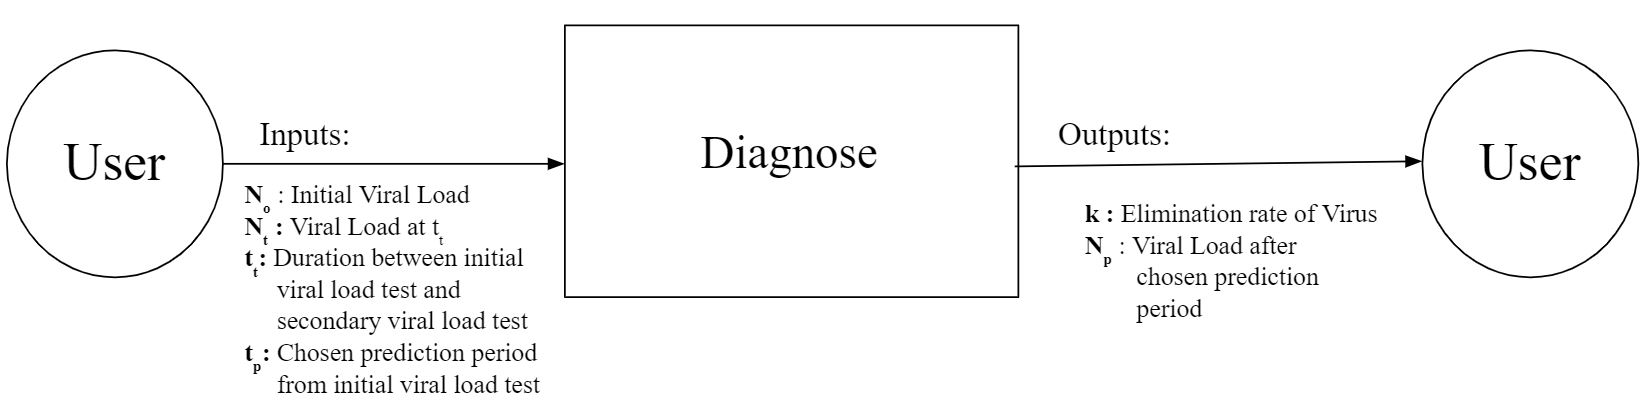
\includegraphics[width=0.6\textwidth]{systemcontext.jpg}
\caption{System Context}
\label{Fig_SystemContext} 
\end{center}
\end{figure}

\begin{itemize}
\item User Responsibilities:
\begin{itemize}
\item Provide viral load data for two consecutive days and patient information, 
including gender and age.
\item Ensure required software assumptions (Section~\ref{sec_assumpt}) are 
appropriate for any particular problem the software addresses.

\end{itemize}
\item diagnosis-AIDs Responsibilities:
\begin{itemize}
\item Assess the input data and determine if the required physical and software 
constraints (Section~\ref{sec_DataConstraints}) are met.
\item Calculate predictions of 30 day viral load concentration.
\end{itemize}
\end{itemize}

\subsection{User Characteristics} \label{SecUserCharacteristics}
\plt{The users of diagnosis-AIDS should be HIV healthcare providers including 
doctors of medicine (MD) or doctors of osteopathic medicine (DO), nurse 
practitioners (NP), or a physician assistant (PA). \citep{cdc}}


\subsection{System Constraints} \label{Sec_constraints}

\plt{The system, diagnosis-AIDs, is limited to only instances where viral load 
is decaying. If 
the viral load is increasing, the immune system has not recognized the intruders 
and a estimation of immune efficiency cannot be found. More specifically, the 
initial viral load must be greater than the viral load on the consecutive day.}

\section{Specific System Description}

\plt{This section presents the problem description, which gives a 
high-level view of the problem to be solved.  This is followed by the solution 
characteristics specification, which presents the assumptions, theories, 
definitions and finally 
the instance models.}


\subsection{Problem Description} \label{Sec_pd}

\plt{AIDs is one of the most serious health challenges in our global community. 
Many individuals infected with HIV visit healthcare facilities with hopes to 
find solutions to manage 
their conditions. A system ensuring accurate and quick characterization of a 
patient’s condition can prove useful in predicting the progression of viruses 
like HIV, and the diagnosis of diseases like AIDs. Using this system, important 
decisions reached by healthcare professionals will be more data-driven and 
quick.

This system could be used to assess risk before substantial immune destruction 
has occurred. The system is intended to predict the viral load at 30 days, 
and predict the patient’s progression to AIDs.

}

\subsubsection{Terminology and Definitions}

\plt{
This subsection provides a list of terms that are used in the subsequent
sections and their meaning, with the purpose of reducing ambiguity and making it
easier to correctly understand the requirements:

\begin{itemize}

\item Virus: Submicroscopic parasites that infect cells. 
\item Virion: A single entire virus particle.
\item Infected cells: Once a virus comes into contact with a host cell, the 
infected cell will begin to undergo viral replication.
\item Viral Replication: Process where infected cells rapidly reproduce the 
genetic material of the virus rather than it’s own 
products\citep{BURRELL201739}.
\item Helper T cells: The cells of the immune system that help activate T cells.
\item T cells: The cells of the immune system that kill infected target cells. A 
common type of T-cell are CD4+ cells.
\citep{william_2018}
\item HIV Virus: HIV infects cells in the immune system.
\item Immune Response: The defensive reaction of the human body against the 
harmful substances like HIV.
\item Viral load:  The amount of virus in your blood
\item Decaying: Physical quantity undergoing a constant decline.
\item Clearance: Physical quantity undergoing a constant decline.
\item AIDs: Acquired Immunodeficiency Syndrome is where the Viral Load increases 
to an extent where the  CD4+ cell count decreases to below 200 
$cells/10^{-3}m^3$.\citep{hiv.gov}
\item Diagnosis: The medical decision determining a patient's condition reached 
by a healthcare professional.
\item Progression: The development towards a more advanced stage.
\item Progression Speed: The rate of developing to a more advanced stage. For 
example, slow, moderate and fast progression.

\end{itemize}

\subsubsection{Physical System Description} \label{sec_phySystDescrip}

\plt{The physical system of diagnosis-AIDs, as seen in 
(Figure~\ref{Fig_PhysicalSystem}), occurs within the human body and includes the 
following elements:}


\begin{itemize}

\item[PS1:] The HIV Virion.

\item[PS2:] An infected cell with the virus.

\item[PS3:] The helper T cells. 

\end{itemize}

 \begin{figure}[h!]
 \begin{center}
 %\rotatebox{-90}
 {
  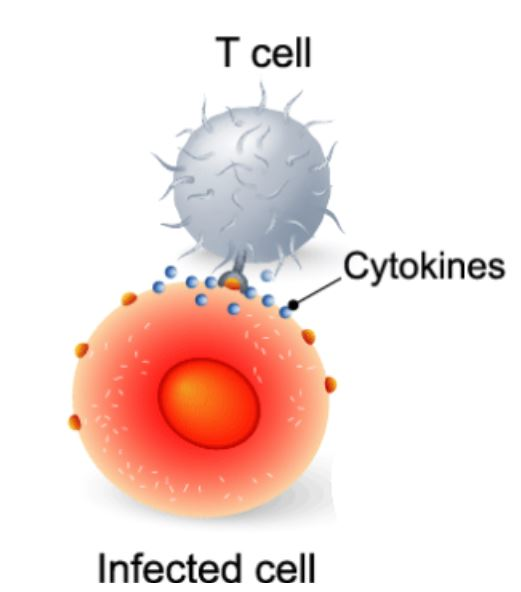
\includegraphics[width=0.5\textwidth]{physicalsystem.jpg}
 }
 \caption{ The Physical System}\citep{wikifig}

 \label{Fig_PhysicalSystem}
 \end{center}
 \end{figure}

\subsubsection{Goal Statements}

\noindent Given two HIV-1 viral load datum taken on consecutive days, the goal 
statements are:

\begin{itemize}

\item[GS\refstepcounter{goalnum}\thegoalnum \label{G_determine-decay-rate}:] 
\plt{determine-decay-rate: Determine the rate of clearance of the HIV virus due 
to immune response.}

\item[GS\refstepcounter{goalnum}\thegoalnum \label{G_predict-VL-30}:] 
\plt{predict-VL-30: Predict Viral Load at 30 days.}

\end{itemize}

\subsection{Solution Characteristics Specification}

\plt{
The instance models that govern diagnosis-AIDs are presented in
Subsection~\ref{sec_instance}.  The information to understand the meaning of the
instance models and their derivation is also presented in Assumptions, 
Theoretical Models, General Definitions and Data Definitions, so that the 
instance
models can be verified.

\subsubsection{Assumptions} \label{sec_assumpt}


\plt{ This section describes the theoretical assumptions that the system will be 
based on. The theoretical models will be easier to understand by explaining 
these assumptions.
}
  
\begin{itemize}

\item[A\refstepcounter{assumpnum}\theassumpnum \label{initial-inf}:]
  \plt{initial-inf: Initial infection of a HIV patient.}

\item[A\refstepcounter{assumpnum}\theassumpnum \label{const-growth}:]
  \plt{const-growth: The virions will invade uninfected cells at a constant 
rate (Ref By: \lcref{LC_artherapy}).}
  
\item[A\refstepcounter{assumpnum}\theassumpnum \label{const-volume}:]
  \plt{const-volume: The dimensions of the location associated with the 
infection remain constant.(Ref By: \ucref{ULC_constant-conditions})}
  
\item[A\refstepcounter{assumpnum}\theassumpnum \label{const-conditions}:]
  \plt{const-conditions: Temperature in the infection location remains constant. 
Higher temperatures boost replication. (Ref By: \aref{const-volume}, 
\ucref{ULC_constant-conditions})\citep{10.1371/journal.ppat.1002792}}

  
\item[A\refstepcounter{assumpnum}\theassumpnum \label{all-productive}:]
  \plt{all-productive: All infected cells are productively infected cells 
meaning there are no infected cells that do not affect other cells. (Ref By: 
\ucref{ULC_constant-conditions})}
  
\item[A\refstepcounter{assumpnum}\theassumpnum \label{always-decay}:]
  \plt{always-decay: Although slight fluctuations in viral load do occur even 
after the peak, it is assumed that there are no significant upwards trends.}
   
\item[A\refstepcounter{assumpnum}\theassumpnum \label{neglect-drugs}:]
  \plt{neglect-drugs: The clearance rate will not be affected by drugs or other 
therapy that may cause faster clearance. (Ref By: \lcref{LC_artherapy})}
  
\item[A\refstepcounter{assumpnum}\theassumpnum \label{neglect-sick}:]
  \plt{neglect-sick: The clearance rate will not be affected by other viruses 
that may cause that may cause slower clearance. }

\item[A\refstepcounter{assumpnum}\theassumpnum \label{decay-proportional-amt}:]
  \plt{decay-proportional-amt: At any point in time, the decay is assumed to be 
proportional to the amount of viruses present. }

\end{itemize}

\subsubsection{Theoretical Models}\label{sec_theoretical}

\plt{This section focuses on the general equations that diagnosis-AIDs is based 
on.
}

~\newline

\noindent
\begin{minipage}{\textwidth}
\renewcommand*{\arraystretch}{1.5}
\begin{tabular}{| p{\colAwidth} | p{\colBwidth}|}
  \hline
  \rowcolor[gray]{0.9}
  Number& T\refstepcounter{theorynum}\thetheorynum  :IsDecaying
\label{T_isDecaying}\\
  \hline
  Label&\bf Determination of Decaying  \\
  \hline
  Equation&  $isDecaying$ = $VL_1 > VL_2$\\
  &\\
  \hline
  Description & $isDecaying$ is the requirement that needs to be satisfied to 
provide a proper estimate. $VL_1$ is the initial viral load. $VL_2$ is the viral 
load after 24 hours. 
&\\
    \hline
  Source & HIV-1 Dynamics in Vivo: Virion Clearance Rate, Infected Life Span and 
Viral 
Generation Time \citep{Perelson1582}
\\
&\\
  \hline
  Ref.\ By & \aref{always-decay} , Subsection~\ref{Sec_constraints}, \rref 
{R_Inputs}\\ 
  \hline
\end{tabular}
\end{minipage}\\
~\newline

%%%%%%%%%%%%%%%%%%% exp decay

\noindent
\begin{minipage}{\textwidth}
\renewcommand*{\arraystretch}{1.5}
\begin{tabular}{| p{\colAwidth} | p{\colBwidth}|}
  \hline
  \rowcolor[gray]{0.9}
  Number& T\refstepcounter{theorynum}\thetheorynum : ExpDecay 
\label{T_ExpDecay}\\
  \hline
  Label&\bf Function of Exponential Decaying \\
  \hline
  Equation&  $N_t$ = $N_{0} e^{-\lambda t}$\\
  \hline
  Description &  The above equation gives the exponential decrease in quantity 
for a certain time $t$ and decay rate $\lambda$.
&\\
&  $N_{0}$ is the initial amount that will undergo an exponential 
decrease. $N_{0}$ is equivalent to $N(t= 0)$.\\
&  $e^x$ is the exponential function. \\
&  $\lambda$ is the decay constant. \\
&  $t$ is the time elapsed from the initial time.\\
&  $N_t$ is the amount after time, $t$, has elapsed.    \\
&\\
  \hline
  Source & \citep{weisstein}
\\
  \hline
  Ref.\ By & \gdref{rate-d}\\
  \hline
\end{tabular}
\end{minipage}\\
~\newline



\subsubsection{General Definitions}\label{sec_gendef}

\plt{This section collects the laws and equations that will be used to build the 
instance models.}

~\newline

\noindent
\begin{minipage}{\textwidth}
\renewcommand*{\arraystretch}{1.5}
\begin{tabular}{| p{\colAwidth} | p{\colBwidth}|}
\hline
\rowcolor[gray]{0.9}
Number& GD\refstepcounter{defnum}\thedefnum : rate-d \label{rate_D}\\
\hline
Label &\bf Concentration Rate law \\
\hline
% Units&$MLt^{-3}T^0$\\
% \hline
&\\
SI Units&\si{$\dfrac{1 / 10^{-3}m^3}{s}$}\\
&\\

\hline
&\\
Equation&$ rate_D = -\dfrac{\Delta A}{\Delta t} = 
-\dfrac{A_{2}-A_{1}}{t_{2}-t_{1}}  $  \\
&\\
\hline
Description &
The Concentration Rate law describes a decaying rate of a substance that is 
directly 
proportional to it's concentration. 
&\\
& $rate_D$ is the time-dependent concentration gradient. 
($\dfrac{1 / 10^{-3}m^3}{s}$).\\
& $\Delta A$ = $A_{2}-A_{1}$ is the change in amount of substance 
($\dfrac{1}{10^{-3}m^3}$).\\
&$\Delta T$= $t_{2}-t_{1}$ is the time elapsed between $A_{2}$ and $A_{1}$ 
(\si{\s}).
&\\
&\\
\hline
  Source & \citep{Fischer6706}
 \\
  \hline
  Ref.\ By & \aref{decay-proportional-amt}, \tref{T_isDecaying}, 
\tref{T_ExpDecay}\\
  \hline
\end{tabular}
\end{minipage}\\


\subsubsection{Data Definitions}\label{sec_datadef}

\plt{This section collects and defines all the data needed to build the instance 
models.}
 
~\newline

\noindent
\begin{minipage}{\textwidth}
\renewcommand*{\arraystretch}{1.5}
\begin{tabular}{| p{\colAwidth} | p{\colBwidth}|}
\hline
\rowcolor[gray]{0.9}
Number& DD\refstepcounter{datadefnum}\thedatadefnum: conc-virus
\label{Concentration}\\
\hline
Label& \bf Viral Load within the body at a given time\\
\hline
Symbol &$VL$\\
\hline
% Units& $Mt^{-3}$\\
% \hline
&\\
  SI Units & $\dfrac{virions}{10^{-3}m^3}$\\
  &\\
  \hline
  &\\
  Equation& $VL = \dfrac{num_{virions}}{volume}$ \\
  &\\
  \hline
  Description & Viral load describes the concentration of the virus within the 
body at certain time $t$.
 & \\ 
& $VL$ is the viral load at a given time ($\dfrac{virions}{10^{-3}m^3}$). \\
& $num_virions$ is the number of virions in the body 
($volume$).\\
& $volume$ is the amount  of three-dimensional space associated with the body 
($10^{-3}m^3$).\\

&\\
  \hline
  Sources& \citep{Fischer6706}
 \\
  \hline
  Ref.\ By & \iref{VLdecay} , \iref{VLat30}\\
  \hline
\end{tabular}
\end{minipage}\\

\subsubsection{Instance Models} \label{sec_instance}    

\plt{  
This section transforms the problem defined in Section~\ref{Sec_pd} into one 
which is expressed in mathematical terms. It uses concrete symbols defined in 
Section~\ref{sec_datadef} to replace the abstract symbols in the models 
identified in Sections~\ref{sec_theoretical} and~\ref{sec_gendef}.

The goals GS ~\ref{G_determine-decay-rate}: determine-decay-rate and GS 
~\ref{G_predict-VL-30}: predict-VL-30 are met by IM: VLdecay and IM:VLat30.
}


~\newline

%Instance Model 1

\noindent
\begin{minipage}{\textwidth}
\renewcommand*{\arraystretch}{1.5}
\begin{tabular}{| p{\colAwidth} | p{\colBwidth}|}
  \hline
  \rowcolor[gray]{0.9}
  Number& IM\refstepcounter{instnum}\theinstnum : VLdecay \label{VLdecay}\\
  \hline
  Label& \bf Using decay rate $\lambda$ to find VL_{30}\\
  \hline
  Input&$VL_1$, $VL_2$, $t$\\
  & The input is constrained so that $VL_1 \geq 0$, $VL_2 \geq 0$, $t \geq 0$
(\aref{A_charge}) and $VL_1 \geq VL_2$ (\aref{A_charge})
\\
  \hline  
  Output& $ \lambda \leq 0 $, such that\\
  &$\frac{dVL}{dt} = - \lambda VL$, \\
  &$\lambda = -VL \frac{dt}{dV}$ \\
 
  \hline
  Description&$\lambda$ is the decay rate of the viral load.\\
  &$\frac{dVL}{dt} =  \dfrac{VL_{2}-VL_{1}}{t_{2}-t_{1}}$ is the change in viral 
load over time.\\
  &$VL_n$ is the viral load at a certain point.\\
  &\\
  \hline
  Sources& \citep{libretexts_2020}

\\
  \\
  \hline
  Ref.\ By & \dref{rate_D}\\
  \hline
\end{tabular}
\end{minipage}\\

%~\newline

  
~\newline
%Instance Model 2

\noindent
\begin{minipage}{\textwidth}
\renewcommand*{\arraystretch}{1.5}
\begin{tabular}{| p{\colAwidth} | p{\colBwidth}|}
  \hline
  \rowcolor[gray]{0.9}
  Number& IM\refstepcounter{instnum}\theinstnum : VLat30 \label{VLat30}\\
  \hline
  Label& \bf Exponential Decaying function relating the viral load and time
 \\
  \hline
  Input&$VL_1$, $\lambda$, $t$ from \iref{epcm}\\
  & The input is constrained so that $t \geq 0$ and $\lambda \leq 0$
 \\
  \hline
  Output&$VL_t$, $VL_t \leq VL_1$, such that\\
  &$VL_t = VL_1 (1- \lambda)^t$\\
   \\
  \hline
  Description& $VL_1$ is the initial viral load.\\
  &$\lambda$ is the decay rate of the viral load.\\
  &$t$ is the time elapsed between $VL_t$ and $ VL_1$.\\
  \\
  \hline
  Sources& \citep{hobbie_roth_1970}
  \\
  \hline
  Ref.\ By & \tref{T_ExpDecay}\\
  \hline
\end{tabular}
\end{minipage}\\

%~\newline


\subsubsection{Input Data Constraints} \label{sec_DataConstraints}    

Table~\ref{TblInputVar} shows the data constraints on the input 
variables.  The column for physical constraints gives the physical limitations
on the range of values that can be taken by the variable.  The column for
software constraints restricts the range of inputs to reasonable values.  The
software constraints will be helpful in the design stage for picking suitable
algorithms.  The constraints are conservative, to give the user of the model the
flexibility to experiment with unusual situations.  The column of typical values
is intended to provide a feel for a common scenario.  The uncertainty column
provides an estimate of the confidence with which the physical quantities can be
measured.  This information would be part of the input if one were performing an
uncertainty quantification exercise.


\begin{table}[!h]
  \caption{Input Variables} \label{TblInputVar}
  \renewcommand{\arraystretch}{1.2}
\noindent \begin{longtable*}{l l l l c} 
  \toprule
  \textbf{Var} & \textbf{Physical Constraints} & \textbf{Software Constraints} &
                             \textbf{Typical Value} & \textbf{Uncertainty}\\
  \midrule 
  $VL_1$ & $VL_1 > 0$ & $VL_1 > VL_2 }$ & $10^6 \frac{virions}{10^{-3}m^3}$ & 
10\%\\
  $VL_2$ & $VL_2 > 0$ & $VL_1 < VL_2 }$ & $10^6 \frac{virions}{10^{-3}m^3}$ & 
10\%\\
  Age &  $Age > 0$ &  $Age > 0$ &  N/A & N/A\\
  \\
  \bottomrule
\end{longtable*}
\end{table}


\subsubsection{Properties of a Correct Solution} \label{sec_CorrectSolution}

\noindent
A correct solution must exhibit a viral load less than the initial viral load 
($VL_1$). 
Table~\ref{TblOutputVar} shows the data constraints for the output variables. 


\begin{table}[!h]
\caption{Output Variables} \label{TblOutputVar}
\renewcommand{\arraystretch}{1.2}
\noindent \begin{longtable*}{l l} 
  \toprule
  \textbf{Var} & \textbf{Physical Constraints} \\
  \midrule 
  $\lambda$ & $\lambda \leq 0 $ 
  \\
  $\VL_30$ & $0 < VL_{30} < VL_2$ 
   \\
  \bottomrule
\end{longtable*}
\end{table}

~\newpage
\section{Requirements}

This section provides the functional requirements, the business tasks that the
software is expected to complete, and the non-functional requirements, the
qualities that the software is expected to exhibit.

\subsection{Functional Requirements}

\noindent \begin{itemize}

\item[R\refstepcounter{reqnum}\thereqnum \label{R_Inputs}:] \plt{R-Inputs: The 
viral load 
concentrations taken on two consecutive days is input. 
(Subsection~\ref{sec_CorrectSolution})}

\item[R\refstepcounter{reqnum}\thereqnum \label{R_Assumptions}:] 
\plt{R-Assumptions: The system 
should set the known numbers within values. }

\item[R\refstepcounter{reqnum}\thereqnum \label{R_Constraints}:] \plt{ 
R-Constraints: AIDsdiagnosis will ensure the input values are not out of bounds 
and are in 
accordance to the data constraints.
Otherwise, an error message will identify the inability of AIDsdiagnosis to 
run.(Ref by: (Subsection~\ref{sec_DataConstraints}))}
    
\item[R\refstepcounter{reqnum}\thereqnum \label{R_AIDsdiagnosis}:] 
\plt{R-AIDsdiagnosis: If all 
constraints are met, the AIDsdiagnosis will output: 30 day viral load 
estimation. (Ref by: \iref{VLat30}, \iref{ProgSpeed})}

\item[R\refstepcounter{reqnum}\thereqnum \label{R_VerifyOutput}:]
  \plt{R-VerifyOutput: The output values will be cross referenced with the 
output constraints 
table to ensure the input values are not out of bounds and are in accordance to 
the results constraints.}

\item[R\refstepcounter{reqnum}\thereqnum \label{R_Output}:] \plt{R-Output: 
Output related
    requirements.}

\end{itemize}


\subsection{Non-functional Requirements}

This section provides the non-functional requirements, the qualities that the 
software is expected to exhibit.

\noindent \begin{itemize}

\item[NR\refstepcounter{nreqnum}\thenreqnum \label{NR_Correctness}:] 
\plt{Correctness: The output values have to adhere to the output properties in 
(Subsection~\ref{sec_CorrectSolution}).}

\item[NR\refstepcounter{nreqnum}\thenreqnum \label{NR_Verifiable}:] 
\plt{Verifiable: The code is tested with a complete verification and validation 
plan.}

\item[NR\refstepcounter{nreqnum}\thenreqnum \label{NR_Usability}:] 
\plt{Usability: The code will consist of several modules to ensure usability.}

\item[NR\refstepcounter{nreqnum}\thenreqnum \label{NR_Understandability}:] 
\plt{Understandability: The code will be completed with a module guide and an 
easy to understand interface.}

\item[NR\refstepcounter{nreqnum}\thenreqnum \label{NR_Maintainability}:] 
\plt{The 
traceability between requirements, assumptions, theoretical models, general 
definitions, data definitions, instance models, likely changes, unlikely 
changes, and modules is completely recorded in traceability matrices in the SRS 
and module guide.}

\end{itemize}


\section{Likely Changes} 

This section lists the likely changes to be made to software   

\noindent \begin{itemize}

\item[LC\refstepcounter{lcnum}\thelcnum\label{LC_time-frame}:] \plt{ Time Frame: 
The program may be expanded to cover a wide range of time frames, greater than 
30 
days.}

\item[LC\refstepcounter{lcnum}\thelcnum\label{LC_progression-acc}:] \plt{ Better 
Progression Accuracy: The program may become more exact in terms of determining 
the time to AIDs.}

\item[LC\refstepcounter{lcnum}\thelcnum\label{LC_artherapy}:] 
\plt{Addition of Therapy: The program may be extended to assess the progression 
due to the patient’s 
immune response as well as the retroviral therapy. (Ref by: 
\aref{neglect-drugs})}

\end{itemize}

\section{Unlikely Changes}    

This section lists the unlikely changes to be made to the software.

\begin{itemize}

\item[UC\refstepcounter{ucnum}\theucnum\label{ULC_determine-decay-rate}:] 
\plt{determine-decay-rate: The goal to simulate the interactions between the 
virions and the immune System cells will remain unchanged. (Ref By: 
\ref{R_Constraints})}

\item[UC\refstepcounter{ucnum}\theucnum\label{ULC_external-input}:] 
\plt{external-input: There will always be a source of input data external to the 
software. (Ref By: R: \ref{R_Inputs})}

\item[UC\refstepcounter{ucnum}\theucnum\label{ULC_constant-conditions}:] 
\plt{constant-conditions: Constant temperature and body conditions are met. (Ref 
by: \aref{const-volume}, \aref{const-conditions})}

\end{itemize}

\section{Traceability Matrices and Graphs}

The purpose of the traceability matrices is to provide easy references on what
has to be additionally modified if a certain component is changed.  Every time a
component is changed, the items in the column of that component that are marked
with an ``X'' may have to be modified as well.  Table~\ref{Table:trace} shows 
the
dependencies of theoretical models, general definitions, data definitions, and
instance models with each other. Table~\ref{Table:R_trace} shows the
dependencies of instance models, requirements, and data constraints on each
other. Table~\ref{Table:A_trace} shows the dependencies of theoretical models,
general definitions, data definitions, instance models, and likely changes on
the assumptions.


\afterpage{
%\begin{landscape}
\begin{table}[h!]
\centering
\begin{tabular}{|c|c|c|c|c|c|c|c|c|c|}
\hline
	& \aref{initial-inf}& \aref{const-growth}& \aref{const-volume}& 
\aref{const-conditions}& 
\aref{all-productive}& \aref{always-decay}& \aref{neglect-drugs}& 
\aref{neglect-sick}& \aref{decay-proportional-amt} \\
\hline
\tref{T_isDecaying}        &X & & & & &X & & &  \\ \hline
\tref{T_ExpDecay}        & &X &X &X &X & &X &X &X  \\ \hline
\dref{rate_D}           & &X &X &X & & & & &X  \\ \hline
\ddref{Concentration}     & &X &X &X &X & & & &X  \\ \hline
\iref{VLdecay}         & &X &X &X &X & & & &X  \\ \hline
\iref{VLat30}         & &X &X &X &X &X & & &X  \\ \hline
\lcref{LC_time-frame}     &X & & & & & & & &  \\ \hline
\lcref{LC_progression-acc}    & & & & &X &X & & &X  \\ \hline
\lcref{LC_artherapy}   & & & & & & &X &X &X  \\ \hline

\hline
\end{tabular}
\caption{Traceability Matrix Showing the Connections Between Assumptions and 
Other Items}

\label{Table:A_trace}
\end{table}
%\end{landscape}
}

\begin{table}[h!]
\centering
\begin{tabular}{|c|c|c|c|c|c|c|}
\hline        
	& \tref{T_isDecaying}& \tref{T_ExpDecay}& \dref{rate_D}& \ddref{Concentration}& 
\iref{VLdecay} & 
\iref{VLat30} \\
\hline
\tref{T_isDecaying}        & & &X & & & \\ \hline
\tref{T_ExpDecay}        & & &X & & &  \\ \hline
\dref{rate_D}           &X &X & & & & \\ \hline
\ddref{Concentration}     & & & & &X &X \\ \hline
\iref{VLdecay}         & & &X &X & &X \\ \hline
\iref{VLat30}         & &X &X &X &X & \\ 
\hline
\end{tabular}
\caption{Traceability Matrix Showing the Connections Between Items of Different 
Sections}
\label{Table:trace}
\end{table}

\begin{table}[h!]
\centering
\begin{tabular}{|c|c|c|c|c|c|c|c|}
\hline
	& \ref{sec_DataConstraints}& \rref{R_Inputs}& 
\rref{R_Assumptions}& \rref{R_Constraints}& \rref{R_AIDsdiagnosis}& 
\rref{R_VerifyOutput}& \rref{R_Output} 
\\
\hline
\iref{VLdecay}         	&X &X &X &X & & & \\ \hline
\iref{VLat30}			&X & &X & &X &X &X  \\ 
\hline
\end{tabular}
\caption{Traceability Matrix Showing the Connections Between Requirements and 
Instance Models}
\label{Table:R_trace}
\end{table}

The purpose of the traceability graphs is also to provide easy references on
what has to be additionally modified if a certain component is changed.  The
arrows in the graphs represent dependencies. The component at the tail of an
arrow is depended on by the component at the head of that arrow. Therefore, if a
component is changed, the components that it points to should also be
changed. 


\newpage

\section{References}

\bibliographystyle {plainnat}
\bibliography{SRSref.bib}

\newpage


\end{document}
